\documentclass{extbook}
\usepackage[papersize={8.5in,11in},top=1in,bottom=1in]{geometry}
\RequirePackage{fix-cm}
\usepackage[T1]{fontenc}
\usepackage{lmodern}
\usepackage{fullpage}
\usepackage{titlesec}
\usepackage{parskip}
\usepackage{float}
\usepackage{url}
\usepackage{hyperref}
\usepackage{graphicx}
\usepackage{tcolorbox}
\usepackage{tabularx}
\usepackage{xcolor}
\usepackage{titlesec}
\usepackage{amsmath}
\usepackage{tcolorbox}
\usepackage{tabularx}

\renewcommand{\contentsname}{Contenido}
\renewcommand{\figurename}{Figura}
\renewcommand{\tablename}{Tabla}
\renewcommand{\listtablename}{Lista de tablas}
\renewcommand{\listfigurename}{Lista de figuras}
\usepackage[fontsize=13.5pt]{fontsize}
\setlength{\parindent}{0pt}

\titleformat{\chapter}[display]
  {\bfseries\huge} % Estilo del título
  {\hfill\Large} % Alineación a la derecha
  {3ex} % Espaciado entre el número del capítulo y el título
  {\vspace{-5cm}\titlerule\vspace{1.5ex}\hfill} % Regla arriba y alineación del título a la derecha
  [\vspace{1ex}\titlerule] % Regla debajo del título


  \makeatletter
  \patchcmd{\chapter}
    {\if@openright\cleardoublepage\else\clearpage\fi}
    {\clearpage}
    {}{}
  \makeatother

  \definecolor{codegreen}{rgb}{0,0.6,0}
  \definecolor{codegray}{rgb}{0.5,0.5,0.5}
  \definecolor{codepurple}{rgb}{0.58,0,0.82}
  \definecolor{backcolour}{rgb}{0.95,0.95,0.92}

\begin{document}
\begin{titlepage}
  \begin{center}
      {\huge \textbf{Universidad Tecnológica de Panamá}}\\
      \vspace{3mm}
      {\Large \textbf{Centro Regional De Veraguas}}

      \begin{figure}[H]
          \centering
          
\includegraphics[scale = 0.07]{Imagenes/utp.png}
          
\includegraphics[scale = 0.58]{Imagenes/fisc.png}
      \end{figure}
      {\Large \textbf{Facultad de Ingeniería de Sistemas Computacionales}}\\
      \vspace{5mm}
      
      {\Large \textbf{Curso: Ingeniería de Sistemas Robóticos}}\medskip
      
      {\Large \textbf{Profesor: Cristian Pinzón}}

      \rule{\linewidth}{0.75mm}\\
          {\Large \textsc{Taller 5}} 
      \rule{\linewidth}{0.75mm}\medskip

      {\Large \textbf{Estudiantes}}\\
      \vspace{5mm}
      {\Large \textbf{Priscila Ortega, Elbin Puga, Arland Barrera}}
      \vfill
      {\Huge \textbf{2024}}

  \end{center}
\end{titlepage}
\tableofcontents
\listoffigures
\listoftables %para lista de tablas 
\chapter{Introducción}
La Jetson NANO de NVIDIA es una plataforma de desarrollo para implementar sistemas de inteligencia artificial cómodamente. Incluye todos los periféricos necesarios para desarrollar un sistema embebido que utilice visión artificial, redes neuronales y más. En esta presentación vamos a estudiar esta placa, sus principales caracteristicas, su uso, precios y más.
\chapter{Desarollo}
\section{¿Qué es?}
NVIDIA Jetson Nano es un producto de NVIDIA que puede implementar soluciones de IoT con el poder de la computación de la GPU. Esta placa tiene pines GPIO y un núcleo de GPU para ayudar a los desarrolladores, creadores y usuarios de TI a crear programas fácilmente.

\begin{figure}[H]
  \centering
  
\includegraphics[scale = 0.3]{Imagenes/nvidia-logo.png}
  \caption{Logo de NVIDIA}{Fuente: Internet}
\end{figure}
\section{Evolución}
A fines de abril de 2014, Nvidia envió la placa de desarrollo Nvidia Jetson TK1 que contenía un SoC Tegra K1 en la variante T124.

\begin{figure}[H]
  \centering
  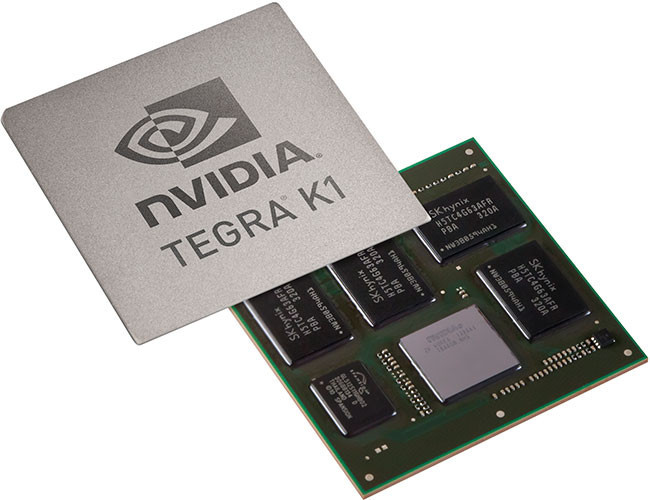
\includegraphics[scale = 0.3]{Imagenes/tegra_k1.jpg}
  \caption{Placa NVIDIA TEGRA K1}{Fuente: Internet}
\end{figure}

La placa de desarrollo Nvidia Jetson TX1 incorpora un Tegra X1 del modelo T210.

La placa Nvidia Jetson TX2 incorpora un Tegra X2 de microarquitectura GP10B. Esta placa y la plataforma de desarrollo asociada se anunciaron en marzo de 2017 como un diseño de tarjeta compacto para escenarios de bajo consumo, por ejemplo, para su uso en drones con cámara más pequeños.

El Nvidia Jetson Xavier se anunció como un kit de desarrollo a fines de agosto de 2018. Se dieron indicios de que se debería esperar una aceleración de 20 veces para ciertos casos de aplicación en comparación con los dispositivos predecesores, y que la eficiencia energética de la aplicación se mejora 10 veces.

\begin{figure}[H]
  \centering
  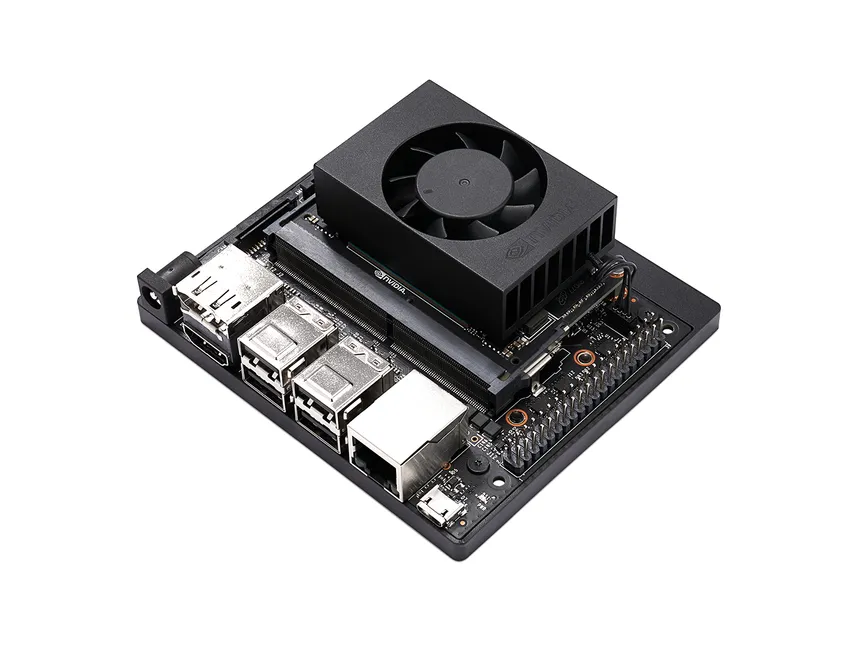
\includegraphics[scale = 0.3]{Imagenes/jetson_xavier.png}
  \caption{Placa NVIDIA Jetson Xavier}{Fuente: Internet}
\end{figure}

El Nvidia Jetson Nano se anunció como un sistema de desarrollo a mediados de marzo de 2019. El mercado previsto es la robótica para aficionados debido a su bajo precio.

\begin{figure}[H]
  \centering
  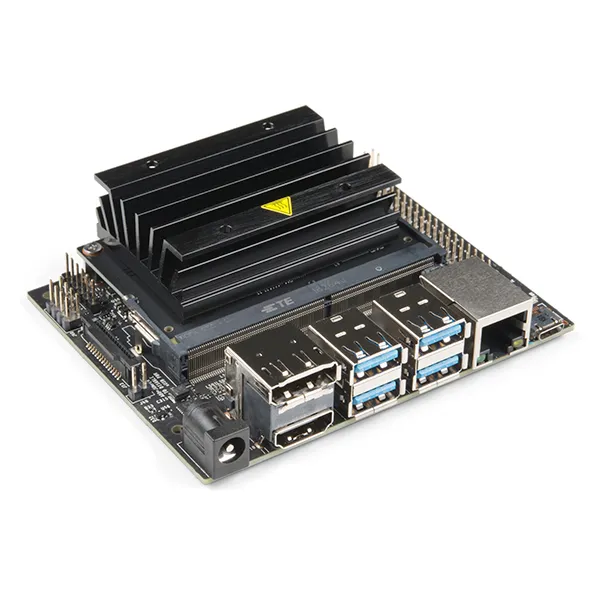
\includegraphics[scale = 0.3]{Imagenes/jetson_nano.png}
  \caption{Placa NVIDIA Jetson Nano}{Fuente: Internet}
\end{figure}

En septiembre de 2022, Nvidia anunció el Jetson Orin Nano.
\section{Funciones}
\begin{itemize}
  \item Permite ejecutar múltiples redes neuronales en paralelo para aplicaciones como clasificación de imágenes, detección de objetos, segmentación y procesamiento de voz.
  \item Permite brindar nuevas e increíbles capacidades a millones de sistemas de IA pequeños y energéticamente eficientes. Abre nuevos mundos de aplicaciones de IoT integradas, que incluyen grabadoras de video en red (NVR) básicas, robots domésticos y puertas de enlace inteligentes con capacidades de análisis completas.
\end{itemize}
\section{Características}
\begin{table}[H]
  \centering
  \begin{tabular}{|c|c|}
      \hline
      GPU & \parbox[c]{13cm}{NVIDIA Maxwell™ architecture with 128 NVIDIA CUDA®\\cores0.5 TFLOPs (FP16)}\\
      \hline
      CPU & Quad-core ARM® Cortex®-A57 MPCore processor\\ 
      \hline
      Memory & 4 GB 64-bit LPDDR41600MHz - 25.6 GB/s\\
      \hline
      Storage & 16 GB eMMC 5.1 Flash\\
      \hline
      Video Encode & \parbox[c]{13cm}{250 MP/sec1x 4K @ 30 (HEVC)2x 1080p @ 60(HEVC)4x 1080p\\@ 30 (HEVC)}\\
      \hline
      Video Decode & \parbox[c]{13cm}{500 MP/sec1x 4K @ 60 (HEVC)2x 4K @ 30 (HEVC)4x 1080p\\@ 60 (HEVC)8x 1080p @ 30 (HEVC)}\\
      \hline
      Camera & \parbox[c]{13cm}{Up to 4 cameras 12 lanes (3x4 or 4x2) MIPI CSI-2DPHY 1.1\\(18 Gbps)}\\
      \hline
      Connectivity & \parbox[c]{13cm}{Wi-Fi requires external chip\\10/100/1000 BASE-T Ethernet}\\
      \hline
      Display & HDMI 2.0 or DP1.2 | eDP 1.4 | DSI (1 x2) 2 simultaneous\\
      \hline
      UPHY & 1 x1/2/4 PCIE, 1x USB 3.0, 3x USB 2.0\\
      \hline
      I/O & 1x SDIO / 2x SPI / 4x I2C / 2x I2S / GPIOs -> I2C, I2S\\
      \hline
      Size & 69.6 mm x 45 mm\\
      \hline
      Mechanical & 260-pin edge connector\\
      \hline
  \end{tabular}
  \caption{Características de la placa NVIDIA Jetson Nano}{Fuente: Internet}
\end{table}
\section{Componentes y esquema}
Elementos de la placa NVIDIA Jetson Nano:

\begin{enumerate}
  \item Ranura para tarjeta microSD para almacenamiento principal.
  \item Cabezal de expansión de 40 pines.
  \item Puerto micro-USB para entrada de alimentación de 5V 2A o para datos.
  \item Puerto Gigabit Ethernet.
  \item Puertos USB 3.0 Tipo A (x4).
  \item Puerto de salida HDMI.
  \item Conector DisplayPort.
  \item Conector Barril DC para entrada de alimentación de 5V 4A.
  \item Conectores de cámara MIPI CSI (compatible con la PiCam).
\end{enumerate}

\begin{figure}[H]
  \centering
  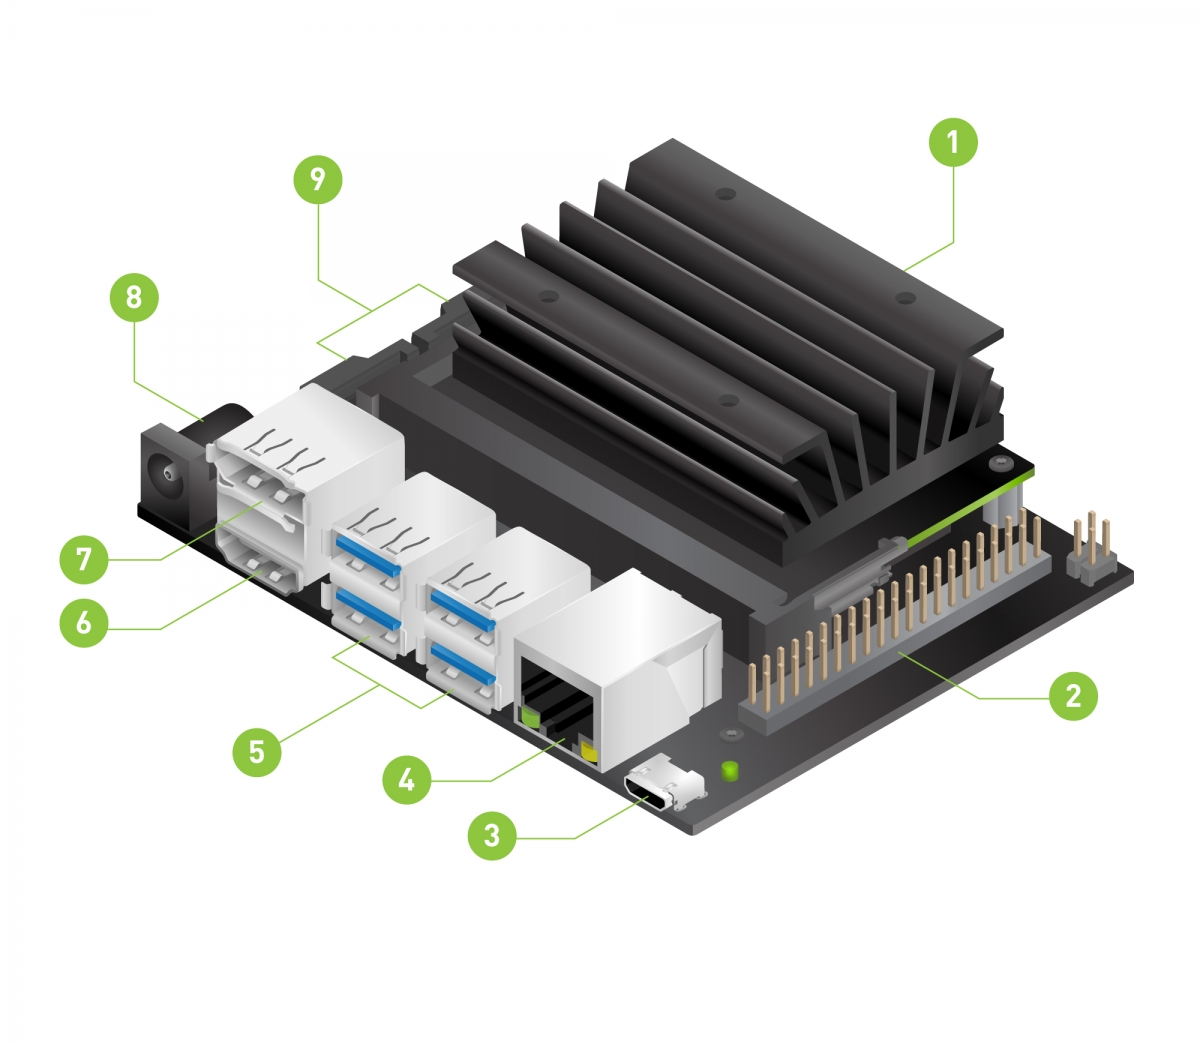
\includegraphics[scale = 0.5]{Imagenes/jetson_nano_esquema.jpg}
  \caption{Esquema de la placa NVIDIA Jetson Nano}{Fuente: Internet}
\end{figure}
\section{Proyectos en los que se utiliza}
\textbf{Detección y Clasificación de Objetos}: Ideal para tareas de visión artificial, la Jetson Nano utiliza frameworks como TensorFlow y PyTorch.

\begin{figure}[H]
  \centering
  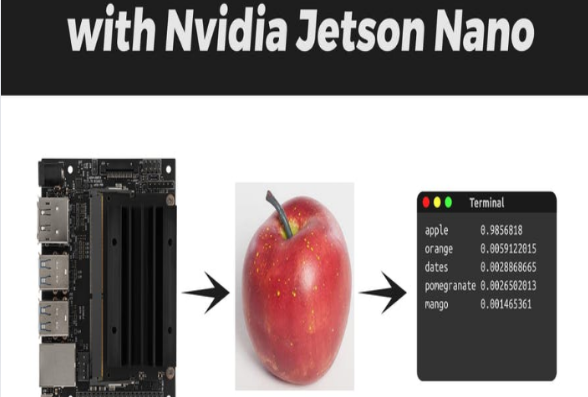
\includegraphics[scale = 0.7]{Imagenes/clasificacion_objetos.png}
  \caption{Detección y extracción de datos}{Fuente: Internet}
\end{figure}

\textbf{Robots Autónomos}: Su capacidad de procesamiento en tiempo real permite a los robots interpretar su entorno, identificar objetos.

\begin{figure}[H]
  \centering
  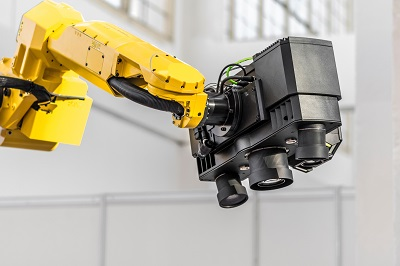
\includegraphics[scale = 1]{Imagenes/jetson_surveillance.jpg}
  \caption{Brazo robot de vigilancia}{Fuente: Internet}
\end{figure}

\textbf{Aplicaciones Médicas}: En el ámbito de la salud, la Jetson Nano facilita el análisis de imágenes médicas.

\begin{figure}[H]
  \centering
  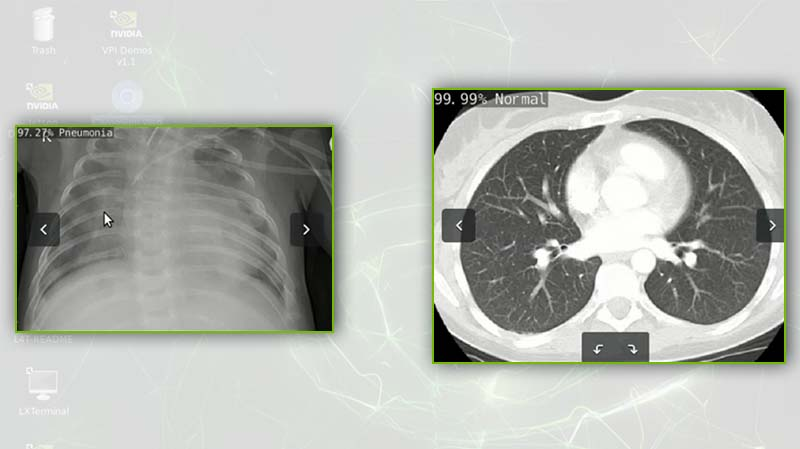
\includegraphics[scale = 0.5]{Imagenes/healthcare.jpg}
  \caption{Análisis de imágenes}{Fuente: Internet}
\end{figure}

\textbf{Proyectos de IoT}: Ideal para aplicaciones de Internet de las Cosas, donde se necesita una toma de decisiones rápida sin depender de la nube, como en el monitoreo ambiental.

\begin{figure}[H]
  \centering
  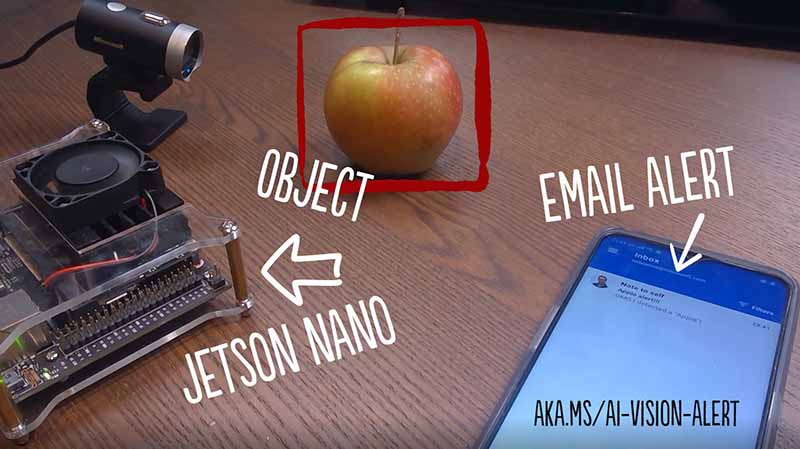
\includegraphics[scale = 0.5]{Imagenes/IoT.jpg}
  \caption{Sistema IoT}{Fuente: Internet}
\end{figure}
\section{Comparación con Arduino Uno}
\begin{table}[H]
  \centering
  \begin{tabular}{|c|c|c|}
      \hline
      Característica & NVIDIA Jetson Nano & Arduino Uno\\
      \hline
      Almacenamiento & 16 GB eMMC 5.1 Flash & \parbox[c]{4cm}{32 KB Flash, sin\\almacenamiento\\externo}\\ 
      \hline
      \parbox[c]{4.5cm}{GPU,\\Interfaz de camara,\\Video Encode/Decode} & Tiene & No tiene\\
      \hline
      CPU & Nvidia Maxwell a 0.5 TFLOPS & AtMega328p\\
      \hline
      Funcionalidad & \parbox[c]{6cm}{Ejecución de aplicaciones complejas (aprendizaje\\profundo, análisis en tiempo real)} & \parbox[c]{4cm}{Proyectos básicos de electrónica\\(encender LEDs, controlar motores)}\\
      \hline
      Uso y Aplicaciones & \parbox[c]{6cm}{Proyectos que requieren procesamiento de imágenes\\e inteligencia artificial} & \parbox[c]{4cm}{Proyectos básicos y educativos sobre\\circuitos y\\programación}\\
      \hline
      Facilidad de Uso & \parbox[c]{6cm}{Más complejo en configuración y mantenimiento;\\requiere conocimientos intermedios} & \parbox[c]{4cm}{Accesible para principiantes;\\amplia documentación y comunidad de apoyo.}\\
      \hline
  \end{tabular}
  \caption{Comparación NVIDIA Jetson Nano y Arduino Uno}{Fuente: Internet}
\end{table}
\section{Costo Estimado}
\begin{figure}[H]
  \centering
  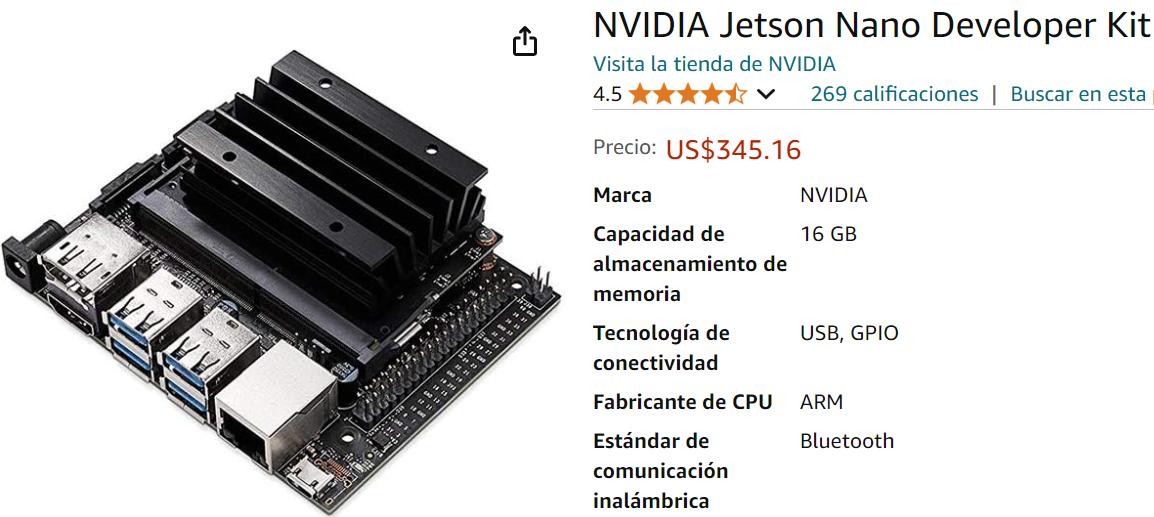
\includegraphics[scale = 0.5]{Imagenes/jetson_nano_amazon.png}
  \caption{NVIDIA Jetson Nano Developer Kit}{Fuente: Internet}
\end{figure}

\begin{figure}[H]
  \centering
  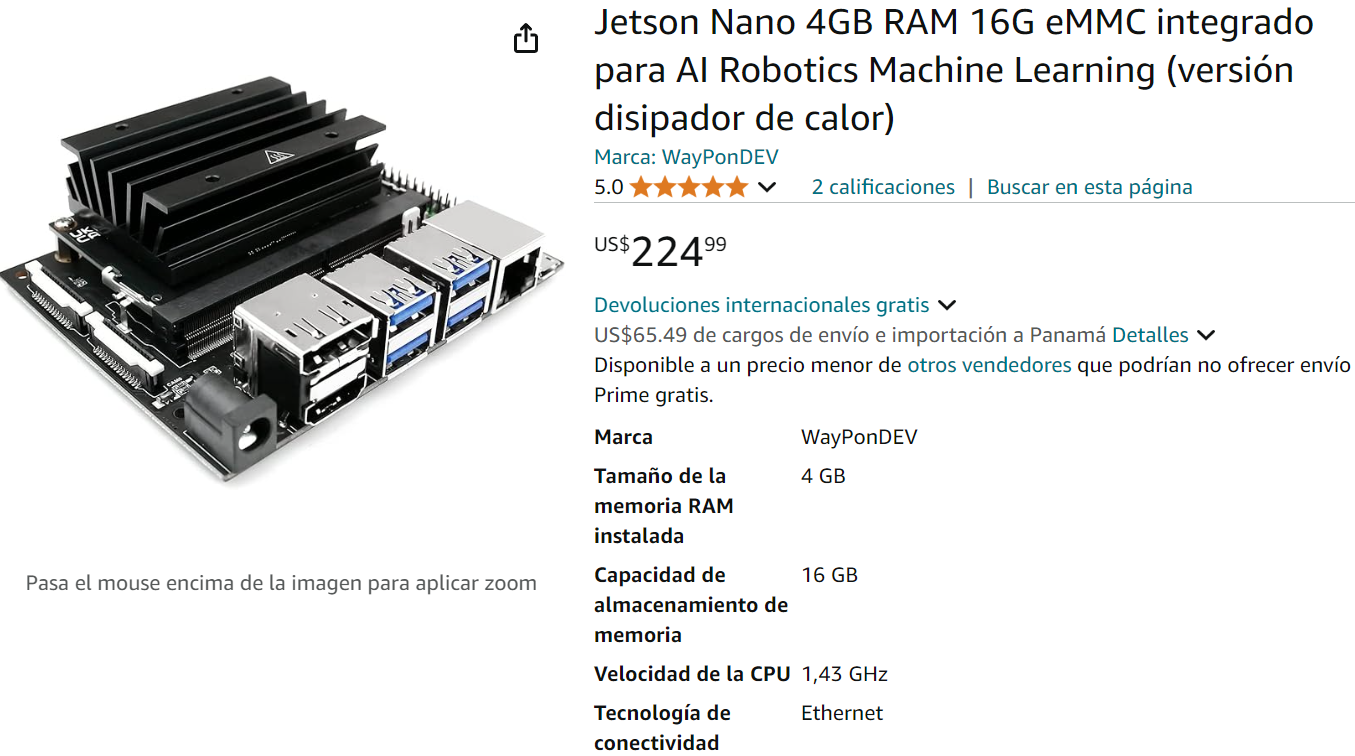
\includegraphics[scale = 0.4]{Imagenes/nano_ai_amazon.png}
  \caption{Jetson Nano AI Robotics Machine Learning}{Fuente: Internet}
\end{figure}
\chapter{Conclusiones}
La NVIDIA Jetson Nano se presenta como una placa potente para abordar una amplia gama de problemas que hay afuera, en la vida cotidiana. En la investigación, nos dimos cuenta que tiene una capacidad barbara para procesar grandes volúmenes de datos en tiempo real, combinada con su soporte para inteligencia artificial y aprendizaje automático, la convierte en una placa ideal para el desarrollo de soluciones innovadoras en diversas áreas.
\chapter{Conclusiones Finales}
Considero que este taller es muy informativo e interesante, pues es curioso conocer otras placas a aparte de la que se utiliza en clase y sus características. Los tecnisismos son interesantes, ya que aportan una visión más detallada o profunda de las placas y sus funcionalidades.
\chapter{Referencias}
\begin{itemize}
  \item Kurniawan, A. (2021). Introduction to NVIDIA Jetson Nano. In: IoT Projects with NVIDIA Jetson Nano. Apress, Berkeley, CA.
  \item Nvidia Jetson \url{https://en.wikipedia.org/wiki/Nvidia_Jetson#cite_note-8}
  \item Jetson Nano \url{https://www.nvidia.com/es-la/autonomous-machines/embedded-systems/jetson-nano/product-development/}
  \item ¿Qué puedo hacer con una Jetson Nano? \url{https://www.330ohms.com/blogs/blog/que-puedo-hacer-con-una-jetson-nano }
  \item Mistral Solutions. (2024, 31 julio). Mistral Blog | NIVIDIA Jetson Applications - NVIDIA Jetson Nano, NVIDIA Jetson TX2 NX, NVIDIA Jetson Xavier NX. \url{https://www.mistralsolutions.com/blog/nvidia-jetson-modules-use-cases-part-2/#:~:text=Jetson%20Nano%20is%20ideal%20for,image%20recognition%2C%20and%20object%20counting.}
  \item Vision alerting system with IoT Edge, Azure Custom Vision and Jetson. (s. f.). NVIDIA Developer. \url{https://developer.nvidia.com/embedded/community/jetson-projects/vision_alerting_system}
  \item AI for Healthcare with Jetson Nano 2GB. (s. f.). NVIDIA Developer. \url{https://developer.nvidia.com/embedded/community/jetson-projects/ai_for_healthcare}
  \item amazon.com: NVIDIA Jetson Nano Developer Kit : Electronics. (2024). Amazon.com. \url{https://www.amazon.com/NVIDIA-Jetson-Nano-Developer-Kit/dp/B07PZHBDKT%E2%80%8C}
  \item amazon.com: Jetson Nano 4GB RAM 16G eMMC integrado para AI Robotics Machine Learning (versión disipador de calor) : Electrónica. (2024). Amazon.com. \url{https://www.amazon.com/-/es/integrado-Robotics-Machine-Learning-disipador/dp/B0B8DMPWJL/ref=pb_allspark_dp_sims_pao_desktop_session_based_d_sccl_2_3/142-2880780-0925111?psc=1%E2%80%8C}
\end{itemize}
\end{document}